\documentclass[a4paper,ngerman,bibtotocliststotoc]{scrartcl}
\usepackage[automark]{scrpage2}
\pagestyle{scrheadings}
\usepackage{multicol}
%\usepackage{multirow}
\usepackage{graphicx}
%\usepackage{caption}
%\usepackage{comment}
%\usepackage{mathdots}
%\usepackage{natbib}
%\usepackage[utf8x]{inputenc}
%\usepackage
\renewcommand*{\titlepagestyle}{empty}
%Mehr Abstand bei Fußnoten
%Hack von Markus Kohm. Gefunden auf:
%<http://groups.google.de/group/de.comp.text.tex/msg/6ab39a8c01a6c06b>
%\newcommand*{\OrigFootnoteRule}{}
%\let\OrigFootnoteRule=\footnoterule
%\newcommand*{\semiflushbottom}{%
%  \raggedbottom%
%    \renewcommand\footnoterule{%
%        \vskip 0pt plus .001fil%
%	    \OrigFootnoteRule}
%
%	    } 
%Ein anderer Hack von Patrick Pommé scheint zu tun
%<http://groups.google.de/group/de.comp.text.tex/msg/a00556927050e1b1>
\renewcommand{\footnoterule}{\vspace{0,25cm} \rule{5cm}{0.4pt}
\vspace{0,25cm}} 
%\usepackage[bottom]{footmisc}
\usepackage{comment}
 \usepackage{lmodern}
% ersetzen
% Was soll das bedeuten? Es hat was mit der Encodierung zu tun, aber
% was? Kann mich jemand aufklären?
\usepackage[T1]{fontenc}
% Zeichensatz einstellen
\usepackage[utf8]{inputenc}
% Paket für mehrere Sprachen in einen Dokument einbinden
% Wird für die "neue deutsche Rechtschreibung" benötigt
\usepackage{babel}
% Pakete für mathematischen Formelsatz einbinden
\usepackage{amsmath}
\usepackage{amssymb}
% Typographie verbessern
\usepackage{microtype}
\usepackage[
hyperfootnotes=true,
bookmarks,
bookmarksopen=true,
bookmarksnumbered=true,
colorlinks={false},
urlcolor={blue},
linkcolor={blue},
citecolor={blue},
pdfstartview={FitH},
pdfauthor={Johannes Starosta <j.starosta@tu-bs.de>}]{hyperref}
%\newcommand*{\teil}[1]{\section*{\setcounter{part}{1} \Huge Teil 
 %   \thepart :  #1}}
\begin{document}%\
      %\subject{TU Braunschweig\\IBR/Distributed Systems}
      \title{Configuring and using the openstack cloud at IBR}
\author{Johannes Starosta <j.starosta@tu-bs.de>}
\date{September 2012}
%\titlehead{
%    \centering
%\includegraphics{logo_tu}\\
%}
\maketitle
\tableofcontents
%\newpage
%      \subject{TU Braunschweig\\IBR/Distributed Systems}
%      \title{Configuring and using the openstack cloud at IBR}
%\author{Johannes Starosta}
%\maketitle
\begin{abstract}
This document describes how you use and administrate the openstack cloud
of the Distributed Systems Group at TU Braunschweig. It also describes
some basic concepts of openstack. \emph{Warning: It's not a replace of
the official documentation, use with caution!}
\end{abstract}
%struktur:
%einführung komponenten, welche clients
%Benutzermanagment-Konzepte und Handhabung
%Zugriff via nova,euca-tools, hyperfox,dashboard
%Image Erzeugung
\section{Introduction}
\label{sec:introduction}
Openstack consist of five modules, which serves different purposes:
\begin{itemize}
\item The Open Stack Compute Infrastructure is provided by the
  nova-daemon. nova is responsible for:
  \begin{itemize}
  \item  Instance life cycle management
  \item Management of compute resources
  \item Networking and Authorization
  \end{itemize}
It also provides a web service API, which can be used to control the
instances. It's compatible with the EC2 API of Amazon Web Services and
can be used by:
\begin{itemize}
\item The nova-pythonclient, the euca2ools or any other EC2 compatible
  client, the Horizon Webinterface of Openstack
\end{itemize}
\item The OpenStack Imaging Service  ist provided by the glance
  daemon. It's used for retrival, lookup and uploading of virtual
  machine images. It can be accessed via the glance CLI client, any
  EC2/S3 compatible client and Horizon
\item OpenStack Object Storage is provided by the Swift daemon. It can
  be acced by the swift CLI tool, Horizizon oder any Amazon S3 compatible client
\item OpenStack Identity Service  (Keystone) is used to set up user
  authentication and authorization. It can be used by using the
  keystone CLI tool.
\end{itemize}
\section{Configuring users and their permissions with the Openstack
  Identity Service (Keystone)}

\subsection{Basic concepts: Users, tenants and roles}
\label{sec:basic-conc-users}
There are three main concepts of Identity user management are in Openstack:
\begin{itemize}
\item Users: Represents a human user (e.g. Alice,Bob) and has associated
  information such as usernae, password and email
\item Tenants: A tenant can be thought of as a project, group, or
  organization (e.G: group1,IBR...) 
\item Roles: A role captures what operations a user is permitted to
  perform in a given tenant.  A user can have different roles in
  different tenants. Here is an example: Imagine the users Alice and
  Bob. Both are members of the tenant IBR, as well as of the tenant
  group1. Now see their roles:\\
  \begin{center}
  \begin{tabular}{c|c|c}
    User & Tenant & Role  \tabularnewline \hline
    Alice &IBR& admin \tabularnewline \hline
    Bob &IBR&Member  \tabularnewline \hline
    Alice&group1&Member \tabularnewline \hline
    Bob&group1&Member
  \end{tabular}  
  \end{center}
  Alice has the role ,,admin'' of the  tenant ,,IBR'' while
  Bob has the role ,,users''. In the tenant ,,group1'' Alice and Bob
  are have the role ''users''. Please note, that ,,admin'' and
  ,,users' are just names, unless you define the permission polices of a
  certain role. The currenty installed police on the Openstack Cloud
  at IBR just defines the roles ,,admin'' and ,,swiftoperator''.
  A user need to have the role ,,admin'' to do some administrative tasks (e.G: Creating
  users...), which should not be allowed for normal users. If a user
  should be given access to the swift object storage service, he
  should get the role ,,swiftoperator''.\\
Note: A user can have several roles for the same tenant:
\begin{center}
  \begin{tabular}{c|c|c}
    User & Tenant & Role  \tabularnewline \hline
    Bob &IBR&Member \tabularnewline \hline
    Bob & IBR&swiftoperator%\tabularnewline 
  \end{tabular}  
  \end{center}
 For further information see Chapter 6, site 76 of \cite{computeadmin}.%TODO: chapter 6, seite 76 of OS compute
                             %administration essex
                             % \item 
\end{itemize}

\subsection{Creating and managing users, tenants and roles}
\label{sec:creat-manag-users}
Now we want to create an user. Given is following scenario:\\
Alice and Bob are students of Eve. Alice and Bob participates in Eves
cloud computing lab. So Eve wants them to work together on a shared
project. They should be able to create custom images, upload them and
run their own cloud instances (thus they need access to compute and
glance). They also should use Swift Object Storage, so they can upload
their documentation to an Object Storage container. Eve decides to
create a tenant ,,cclab-group1'' for them. Eve wants to have acces to
the tenants instances as well. She also wants to 
have access to the
tenant as well and she wants, administrative permissions, while Alice and Bob shall be
just normal users... So she want to create following
setup:

\begin{center}
  \begin{tabular}{ccc}
    User & Tenant & Role\\
    Alice&cclab-group1&Member\\
    Bob  &cclab-group1&Member\\
    Alice&cclab-group1&swiftoperator\\
    Bob  &cclab-group1&swiftoperator\\
    Eve  &cclab-group1&admin\\
  \end{tabular}
\end{center}

\label{warning}
\label{sec:creat-manag-users-1}


\fbox{\parbox{\textwidth
  }{\begin{center}\LARGE{\textbf{WARNING:}}\end{center}
\emph{The environment on
  cloud2 is configured to do administrative tasks. Don't use it to do
  things, you want to use with a certain user! For example if you
  create an virtual machine instance as user ,,admin'', you won't be
  able to access it from your normal user account. In section
  \ref{sec:using-comp-infr} %TODO reference
                                %to usage chapter} %TODO reference
                                %to usage chapter
   we'll discuss how to access your user environment without messing up
  with the admin account.}}}% \hfill

She connects to \verb|cloud2.ibr.cs.tu-bs.de| and run following
commands in the admin console\footnote{These are NOT real data
  ids. Don't use them in the real world!}
\begin{verbatim}
# Every line, which starts with a # is a comment
# First she wants to know, which users, roles and tenants alreday
#exists
eve@uncinus:~$ keystone user-list
+----------------------------------+---------+-------------------------+-----------+
|                id                | enabled |          email          |    name   |
+----------------------------------+---------+-------------------------+-----------+
| 1f53b11a2e0e40239b25961380472c54 |   True  |  admin@ibr.cs.tu-bs.de  |   swift   |
| 552bfa0c2d6847b6a8ea2625bff5531f |   True  |  admin@ibr.cs.tu-bs.de  |   glance  |
| cfb1870fc4c84a56bd1f19a5e577d984 |   True  |  admin@ibr.cs.tu-bs.de  |    nova   |
| dd69242cbdb243dd803b7641c223adb4 |   True  |  admin@ibr.cs.tu-bs.de  |   admin   |
| eveIDint                         |   True  |   eve@ibr.cs.tu-bs.de   |    eve    |
+----------------------------------+---------+-------------------------+-----------+
eve@uncinus:~$
eve@uncinus:~$ keystone tenant-list
+----------------------------------+----------+---------+
|                id                |   name   | enabled |
+----------------------------------+----------+---------+
| 0b6336de185a4f01a59fcb5ef9f40d96 | service  |   True  |
| 9f4b31c709b2431b972666100cf12c79 |  users   |   True  |
| fa188ad427e24bb6b14b4945fc6af6da |  admin   |   True  |
+----------------------------------+----------+---------+
eve@uncinus:~$ keystone role-list
+----------------------------------+---------------+
|                id                |      name     |
+----------------------------------+---------------+
| 2a292fb8580e49c095059a7b258b57f3 | swiftoperator |
| 45649d6a8b044f1d860905a896b3473b |     Member    |
| 47870520359d4f6b9d5d87a175a2f1f1 |     admin     |
+----------------------------------+---------------+
eve@uncinus:~$
# We already have all needed roles, eve still need to create the
# users, tenant and assign them to the needed roles
eve@uncinus:~$ keystone user-create --name bob --email bob@ibr.cs.tu-bs.de 
                                    --pass bobpass
+----------+-------------------------------------------------------------------------------------------------------------------------+
| Property |                                                          Value                                                          |
+----------+-------------------------------------------------------------------------------------------------------------------------+
|  email   |                                                   bob@ibr.cs.tu-bs.de                                                   |
| enabled  |                                                           True                                                          |
|    id    |                                                        bobsIDint                                                           |
|   name   |                                                           bob                                                           |
| password | $6$rounds=40000$0p.sAOcBsq8ms/Sk$B/yUdMQoxAwpM8kB1RwyHuL.mYrLI/BZZxlrDeT1U.Rm6QfmBn5/MA86KcBHz90Hr67bOV8EGdfUbOkJ0JwBW. |
| tenantId |                                                           None                                                          |
+----------+-------------------------------------------------------------------------------------------------------------------------+
eve@uncinus:~$ keystone user-create --name alice --email alice@ibr.cs.tu-bs.de --pass alicepass
+----------+-------------------------------------------------------------------------------------------------------------------------+
| Property |                                                          Value                                                          |
+----------+-------------------------------------------------------------------------------------------------------------------------+
|  email   |                                                 alice@ibr.cs.tu-bs.de                                                   |
| enabled  |                                                           True                                                          |
|    id    |                                                        aliceIDint                                                       |
|   name   |                                                         alice                                                           |
| password | $6$rounds=40000$0p.sAOcBsq8ms/Sk$B/yUdMQoxAwpM8kB1RwyHuL.mYrLI/BZZxlrDeT1U.Rm6QfmBn5/MA86KcBHz90Hr67bOV8EGdfUbOkJ0JwBW. |
| tenantId |                                                           None                                                          |
+----------+-------------------------------------------------------------------------------------------------------------------------+
#now eve creates the tenant
eve@uncinus:~$ keystone tenant-create  --name cclab-group1
+-------------+----------------------------------+
|   Property  |              Value               |
+-------------+----------------------------------+
| description |               None               |
|   enabled   |               True               |
|      id     | 898daab4fc4d45b98f231872241458e4 |
|     name    |           cclab-group1           |
+-------------+----------------------------------+
eve@uncinus:~$ 
# at the end we assign the needed roles to every user
#eve got role admin
eve@uncinus:~$ keystone user-role-add --user eveIDint  
                        --role 47870520359d4f6b9d5d87a175a2f1f1 
                       --tenant_id 898daab4fc4d45b98f231872241458e4
#bob and alice got the role Member
eve@uncinus:~$ keystone user-role-add --user bobIDint 
                        --role 45649d6a8b044f1d860905a896b3473b 
                       --tenant_id 898daab4fc4d45b98f231872241458e4
eve@uncinus:~$ keystone user-role-add --user aliceIDint 
                        --role 45649d6a8b044f1d860905a896b3473b 
                       --tenant_id 898daab4fc4d45b98f231872241458e4
#bob and alice got the role swiftoperator
eve@uncinus:~$ keystone user-role-add --user bobIDint    
                       --role 2a292fb8580e49c095059a7b258b57f3 
                       --tenant_id 898daab4fc4d45b98f231872241458e4
eve@uncinus:~$ keystone user-role-add --user aliceIDint  
                       --role 2a292fb8580e49c095059a7b258b57f3 
                       --tenant_id 898daab4fc4d45b98f231872241458e4
\end{verbatim}
Now everything ist configured. Of course Eve could have add additional
roles or more tenants. More information how to do identify managment
can be found in chapter 6 of \cite{computeadmin}%For background information refer to
% FIXME referenz einfügen.

\subsection{Updating user information}
\label{sec:updat-user-inform}
You might want to change details of the users. Again we look in our
scenario:
Bob complains, that he can't remember his password. He prefers to have
the password ,,swordfish''. He also would prefered to have another email
(bob@tu-bs.de) in the user-details.
Again Eve connects to \verb|clou2.ibr.cs.tu-bs.de|:
\begin{verbatim}
eve@uncinus:~$
eve@uncinus:~$ keystone user-update --email bob@tu-bs.de bobIDint
eve@uncinus:~$ keystone user-password-update --pass swordfish bobIDint
\end{verbatim}
You can change the details of names and roles as well. 
% FIXME

\subsection{Removing everything}
\label{sec:removing-everything}
Now the term is finished. Alice and Bob have finished their project and
passed the examination. Eve now wants to removes their user-account,
tenant, since the Cloud will be needed for new students next term:
\begin{verbatim}
#first eve remove the roles from the tenant
eve@uncinus:~$ keystone user-role-remove --user eveIDint    
                       --role 47870520359d4f6b9d5d87a175a2f1f1 
                       --tenant_id 898daab4fc4d45b98f231872241458e4
eve@uncinus:~$ keystone user-role-remove --user bobIDint    
                       --role 45649d6a8b044f1d860905a896b3473b 
                       --tenant_id 898daab4fc4d45b98f231872241458e4
eve@uncinus:~$ keystone user-role-remove --user aliceIDint  
                       --role 45649d6a8b044f1d860905a896b3473b 
                       --tenant_id 898daab4fc4d45b98f231872241458e4
eve@uncinus:~$ keystone user-role-remove --user bobIDint    
                       --role 2a292fb8580e49c095059a7b258b57f3 
                       --tenant_id 898daab4fc4d45b98f231872241458e4
eve@uncinus:~$ keystone user-role-remove --user aliceIDint  
                       --role 2a292fb8580e49c095059a7b258b57f3 
                       --tenant_id 898daab4fc4d45b98f231872241458e4
# now we remove the tenant:
eve@uncinus:~$ keystone tenant-delete  898daab4fc4d45b98f231872241458e4
# and in the end the accounts of alice and bob
eve@uncinus:~$ keystone user-delete aliceIDint
eve@uncinus:~  keystone user-remove bobIDint
\end{verbatim}
%TODO Referenz 
%\newpage
%\begin{multicols}{2}

\section{Using the compute infrastructure}
\label{sec:using-comp-infr}

As already mentioned in \ref{warning} you should not use
the environment of the admin user to create new images or
instances. Instead you should connect from a client. You can connect
via the native openstack client tools(nova-pythonclient,glance,swift etc), any EC2-compatible tool, the HybridFox
Firefox Plugin or the Horizon Dashboard. We will describe now how to
configure the clients, before describing how to use them.\\
\subsection{Configuring the native tools}
\label{sec:conf-nova-pyth}
Open a web browser and connect to
\url{http://cloud2.ibr.cs.tu-bs.de}. You should see the login page of
the Horizon dasboard. Login with your username and password
(e.G. Alice, alicepass). Open the subpage ,,Settings''. Open
,,OpenStack Credentials''. Select the project you want to work on and
click ,,Download RC file''. The browser will start do download a file,
called \verb|openrc.sh|. The native tools are configured  by setting
environment variables, e.G. ,,OS\_PASSWORD''.  Thus, you need to source
the file ,,openrc.sh'' before you can use the native tools:
\begin{verbatim}
# source openrc.sh
alice@izcip01:~$ source openrc.sh
Please enter your OpenStack Password:
alice@izcip01:~$
\end{verbatim}
If you don't like the idea of always retyping the password, open
\verb|openrc.sh| in your favourite text editor and change the last lines
to look like this:
\begin{verbatim}
# With Keystone you pass the keystone password.
#echo "Please enter your OpenStack Password: "
#read -s OS_PASSWORD_INPUT
#export OS_PASSWORD=$OS_PASSWORD_INPUT
export OS_PASSWORD=yourpassword
\end{verbatim}
However you still need to source \verb|openrc.sh| everytime you want to
access the cloud. If you have enough of it, you can configure your
UNIX shell, to source \verb|openrc.sh| every time you login to your
UNIX account:
\begin{verbatim}
# First change openrc.sh like described above, so you not getting asked
# for the password
# Make sure, that openrc.sh can be found by the shell:
alice@izcip01:~$ mv openrc.sh .novarc
# open the file .bashrc in your home directory in your favourite text
# editor and add following line to it
source ~/.novarc
#logout and login again, to activate the changes
#test it
alice@izcip01:~$ nova absolute-limits
+--------------------+-------+
|        Name        | Value |
+--------------------+-------+
|    maxImageMeta    |  128  |
|   maxPersonality   |   5   |
| maxPersonalitySize | 10240 |
|   maxServerMeta    |  128  |
|   maxTotalCores    |   20  |
| maxTotalInstances  |   10  |
|  maxTotalRAMSize   | 51200 |
+--------------------+-------+
\end{verbatim}
Now you should be able to use the native tools every time you login to
your UNIX-account.
\subsection{Creating and running instances}
\label{sec:creat-runn-inst}
We need to do following steps, to get a cloud instance to work:
\begin{enumerate}
\item Create and upload a virtual machine image
\item Create a public keypair
\item Run a virtual machine instance
\item Assign a public IP Address to the instance (optional)
\end{enumerate}
Please note, that although step 4 is optional, in reality the virtual machine is nearly useless without
a public IP. Without a public IP, the services provided by the virtual
machine, can not be accessed. 

\subsubsection{Uploading virtual machine images}
\label{sec:create-uplo-virt}
Since the creation of virtual machine images is quite complex, I put
the details in a seperate section \ref{sec:creating-images} on page
\pageref{sec:creating-images}. So let's assume you have already created an
image or just downloaded one of the ready Images from
\url{http://cloud-images.ubuntu.com/}. 
To add the image test.img to the cloud we upload it using the glance
command line tool:
\begin{verbatim}
alice@izcip01:~$ glance add disk_format=qcow2  container_format=ovf name="test" <test.img
=====================[100%] 145.932926M/s, ETA  0h  0m  0s
Added new image with ID: 3d183184-5fa7-475e-bacd-6e78c5e8c245
# note: disk_format shall be in the image format of the uploaded
# image, container_format is the format, which openstack will use to
# store. More information is provided in the section about creating images
alice@izcip01:~$
alice@izcip01:~$ glance index 
ID                                   Name                           Disk Format          Container Format     Size          
------------------------------------ ------------------------------ -------------------- -------------------- --------------
3d183184-5fa7-475e-bacd-6e78c5e8c245 test                            qcow2                ovf                       230490112
\end{verbatim}

\subsection{Create a public keypair}
\label{sec:create-publ-keyp}
We need to create a public keypair. It's used to provide ssh access to
UNIX images.
\begin{verbatim}
alice@izcip01:~$ ssh-keygen 
Generating public/private rsa key pair.
Enter file in which to save the key (/home/alice/.ssh/id_rsa):
Your public key has been saved in dd.pub.
The key fingerprint is:
d6:e2:37:41:02:76:4b:9f:53:e6:f9:a7:36:65:8b:e4 jstarosta@uncinus
The key's randomart image is:
+--[ RSA 2048]----+
|      o o   o    |
|     . + o = .   |
|        o = o    |
|         + . .   |
|        S o  .. +|
|       o . .o .=.|
|        . o  E+. |
|         . . . . |
|                 |
+-----------------+
alice@izcip01:~$ nova keypair-add --pub_key .ssh/id_rsa.pub cloudkey
alice@izcip01:~$ nova keypair-list
+----------+-------------------------------------------------+
|   Name   |                   Fingerprint                   |
+----------+-------------------------------------------------+
| cloudkey | c2:df:5d:2d:ce:a6:64:af:08:64:fa:9a:c5:9f:27:19 |
+----------+-------------------------------------------------+
\end{verbatim}
\subsubsection{Run a virtual machine instance}
\begin{verbatim}
alice@izcip01:~$ nova boot --flavor m1.tiny --image 3d183184-5fa7-475e-bacd-6e78c5e8c245 --key_name cloudkey "testinstance"
+------------------------+--------------------------------------+
|        Property        |                Value                 |
+------------------------+--------------------------------------+
| OS-DCF:diskConfig      | MANUAL                               |
| OS-EXT-STS:power_state | 0                                    |
| OS-EXT-STS:task_state  | scheduling                           |
| OS-EXT-STS:vm_state    | building                             |
| accessIPv4             |                                      |
| accessIPv6             |                                      |
| adminPass              | zS335ooJBMT4                         |
| config_drive           |                                      |
| created                | 2012-10-01T04:12:14Z                 |
| flavor                 | m1.tiny                              |
| hostId                 |                                      |
| id                     | 24d96fdd-55c2-4440-b096-f31aaa148966 |
| image                  | bla                                  |
| key_name               | cloudkey                             |
| metadata               | {}                                   |
| name                   | testinstance                         |
| progress               | 0                                    |
| status                 | BUILD                                |
| tenant_id              | fa188ad427e24bb6b14b4945fc6af6da     |
| updated                | 2012-10-01T04:12:14Z                 |
| user_id                | dd69242cbdb243dd803b7641c223adb4     |
+------------------------+--------------------------------------+
#get a coffe, building the virtual machine take some time
alice@izcip01:~$ nova list
+--------------------------------------+-----------------+--------+-------------------------------------+
|                  ID                  |       Name      | Status |               Networks              |
+--------------------------------------+-----------------+--------+-------------------------------------+
| 24d96fdd-55c2-4440-b096-f31aaa148966 | testinstance    | ACTIVE | private=192.168.4.37                |
+--------------------------------------+-----------------+--------+-------------------------------------+
\end{verbatim}
\subsubsection{Assign a public IP Address to the instance}
A new virtual machine instance get's automatically a private IP from
the subnet 192.168.4.2/27 It's used for communication with other
instances and the hypervisor. However if we want to access a certain
instance from other servers, it needs to get a public IP assigned. 
The IBR network has a subnet 134.169.35.2/27 which provides a pool of
public IPs for openstack:
\begin{verbatim}
# allocate a floating-ip from the pool
alice@izcip01:~$ nova floating-ip-create
+---------------+-------------+----------+------+
|       Ip      | Instance Id | Fixed Ip | Pool |
+---------------+-------------+----------+------+
| 134.169.35.12 | None        | None     | nova |
+---------------+-------------+----------+------+
#assign floating ip to the virtual machine instance with name "testinstance"
lice@izcip01: ~$ nova add-floating-ip testinstance 134.169.35.12
jstarosta@uncinus:~$ nova list
+--------------------------------------+-----------------+--------+-------------------------------------+
|                  ID                  |       Name      | Status |               Networks              |
+--------------------------------------+-----------------+--------+-------------------------------------+
| 24d96fdd-55c2-4440-b096-f31aaa148966 | testinstance    | ACTIVE | private=192.168.4.37, 134.169.35.12 |
+--------------------------------------+-----------------+--------+-------------------------------------+
# allow ssh and pings to the instance
alice@izcip01:~$ nova secgroup-add-rule default icmp -1 -1 0.0.0.0/0
alice@izcip01:~$ nova secgroup-add-rule default tcp 22 22 0.0.0.0/0

\end{verbatim}
\subsubsection{Terminating instances and cleanup the environment}
At some point you'll propably want to deassign public IP, terminate
instances or remove images.
To remove a public IP from a certain instance (e.G. to use it with
another one):
\begin{verbatim}
alice@izcip01:~$ nova remove-floating-ip testinstance 134.169.35.12
\end{verbatim}
To deassociate a public IP (e.G if the users run out of them):
\begin{verbatim}
alice@izcip01:~$ nova floating-ip-delete  134.169.35.12
\end{verbatim}
Terminate and delete an instance:
\begin{verbatim}
alice@izcip01:~$ nova delete testinstance
# if you have more than one instance with the same name 
# use nova delete serverId (as printed from nova list)
\end{verbatim}
Remove an obsolete image:
\begin{verbatim}
alice@izcip01:~$ glance index
ID                                   Name                           Disk Format          Container Format     Size          
------------------------------------ ------------------------------ -------------------- -------------------- --------------
3d183184-5fa7-475e-bacd-6e78c5e8c245 bla                            qcow2                ovf                       230490112
alice@izcip01:~$ glance delete 3d183184-5fa7-475e-bacd-6e78c5e8c245
Delete image 3d183184-5fa7-475e-bacd-6e78c5e8c245? [y/N] y
Deleted image 3d183184-5fa7-475e-bacd-6e78c5e8c245
\end{verbatim}
\subsection{Configuring the euca2ools}
\label{sec:conf-euca2}
Using the native tools is fine, there is however a problem: In the
workstation pool of the Braunschweig Computer Science center (roomz
IZG40) they are not installed, only the euca2ools. It's not a big
deal, since Openstack is compatible with the EC2 API. We just need to
to some preparing work.\\\\
Open a web browser and connect to
\url{http://cloud2.ibr.cs.tu-bs.de}. You should see the login page of
the Horizon dasboard. Login with your username and password
(e.G. Alice, alicepass). Open the subpage ,,Settings''. Open
,,OpenStack Credentials''. Select the project you want to work on and
click ,,Download RC file''. The browser will start do download a
ZIP-Archive with a random name. Now open a shell and type following
commands:
\begin{verbatim}
alice@izcip01:~$ mkdir ~/.euca
alice@izcip01:~$ cd ~/.euca
alice@izcip01:~$ unzip pathto_archiv.zip
alice@izcip01:~$ mv ec2rc.sh eucarc
# euca2ools need S3_URL, which is not defined 
# (Openstack Bug https://bugs.launchpad.net/horizon/+bug/987678)
alice@izcip01:~$ echo "export S3_URL=http://cloud2.ibr.cs.tu-bs.de:3333" >>eucarc
#source eucarc automatically at the login
alice@izcip01:~$ echo "source ~/.euca/eucarc" >>~/.bashrc
#test the setup
alice@izcip01:~$ euca-describe-regions
REGION  nova    http://cloud2.ibr.cs.tu-bs.de:8773/services/Cloud
\end{verbatim}

\subsection{Creating and running instances with the euca2ools}
\label{sec:creat-runn-inst-ec2}
Warning: This is just a short description, taken from Johannes Behls
and Klaus Stengels slides for the Cloud Computing Lecture in summer
ter 2012. It's not complete!

\subsubsection{Preparing the virtual machine image}
\label{sec:prep-virt-mach}


\begin{verbatim}
# create an image  image.raw as described 
# creating the VM-Package (Bundle)                                 "
$ euca - bundle -image -i image.raw -d . --arch i386
# sent VM-Package to OPenstackCloud
# note: The Bucketname doesn't really matter, pick one you like :)
$ euca-upload-bundle -b  <bucket_name> -m image.raw.manifest.xml
# Register the bundle
$ euca-register <bucket_name>/image.raw.manifest.xml 
# List own, registred VM bundles
$ euca-describe-images -o <user>
# Modify an image attributes 
$ euca - modify - image - attribute -l -r all < vm_id >
# removing an VM bundle
$ euca-deregister <vm_id >
$ euca-delete -bundle -b <bucket_name>
\end{verbatim}

\subsubsection{Running the virtual machine}
\label{sec:runn-virt-mach}
\begin{verbatim}
$ euca-run-instances [-t <type>] [ -n <numbers_of_instances>] <vm_id>
#output:  ID of instance(s) (instance id)
# Get the status of the instance (state and IP)
$ euca-describe-instances  
# terminate instance
$ euca - terminate - instances < instanz_id >
\end{verbatim}
Note: This is NOT a complete guide, please refer to the euca2ools
guide \cite{eucatools} on \url{http://open.eucalyptus.com/wiki/Euca2oolsGuide}.
\subsection{Configuring and using Hybridfox}
\label{sec:conf-hybr}
Hybridfox is a Firefox Add-On, which provides a GUI for several tasks
related with cloud computing. It can be downloaded from
\url{http://code.google.com/p/hybridfox/}. 
After installation it can be found in the Menu ,,Extras''.
%At the first start it ask for the user credentials:
We need to add an
additional region before we can set up the credentials:%use Hybridfox
                                %with the IBR-Cloud:
\begin{center}
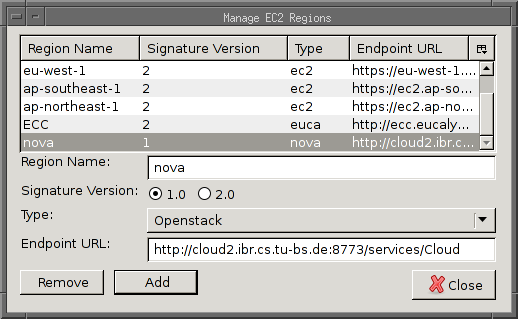
\includegraphics{hybridfox_regions}
\end{center}
Now we setup the credentials:
\begin{center}
  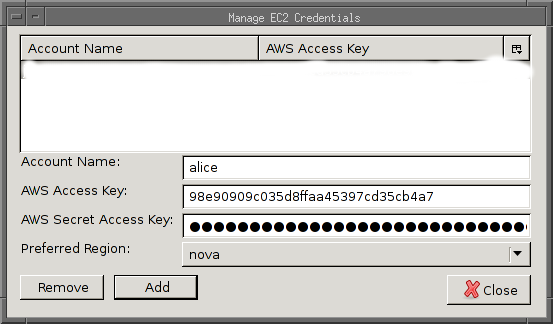
\includegraphics{hybrid_creds}
\end{center}
Setting up images and instances is quite easy. More information
concerning this, can be found in the the Hybridfox User Manual \cite{hybridfoxMan}
\url{http://hybridfox.googlecode.com/files/Hybridfox_User_Manual_v1.pdf}

\section{Creating images}
\label{sec:creating-images}
When we introduced the ,,glance'' command line tool for uploading
images, we didn't explain how to 

\end{document}
